\subsection{La red de tres FPGA}
\label{sec:red}

Una mochila que detecta sola no le dice al rescatista dónde cavar, y su radio no atraviesa el
concreto (sección~\ref{sec:deteccion}). La red resuelve las dos cosas con lo que ya hay en el
escombro: otra mochila. Dos mochilas que ven a la misma persona desde lugares distintos
bastan para ubicarla, y la que quedó cerca de la entrada retransmite el aviso de la que quedó
lejos. La demostración usa tres DE10-Lite (figura~\ref{fig:tresfpga}): dos hacen de mochilas
de dos insectos, A y B, y la tercera es el receptor del operador, en la entrada del derrumbe.

\begin{figure}[H]
\centering
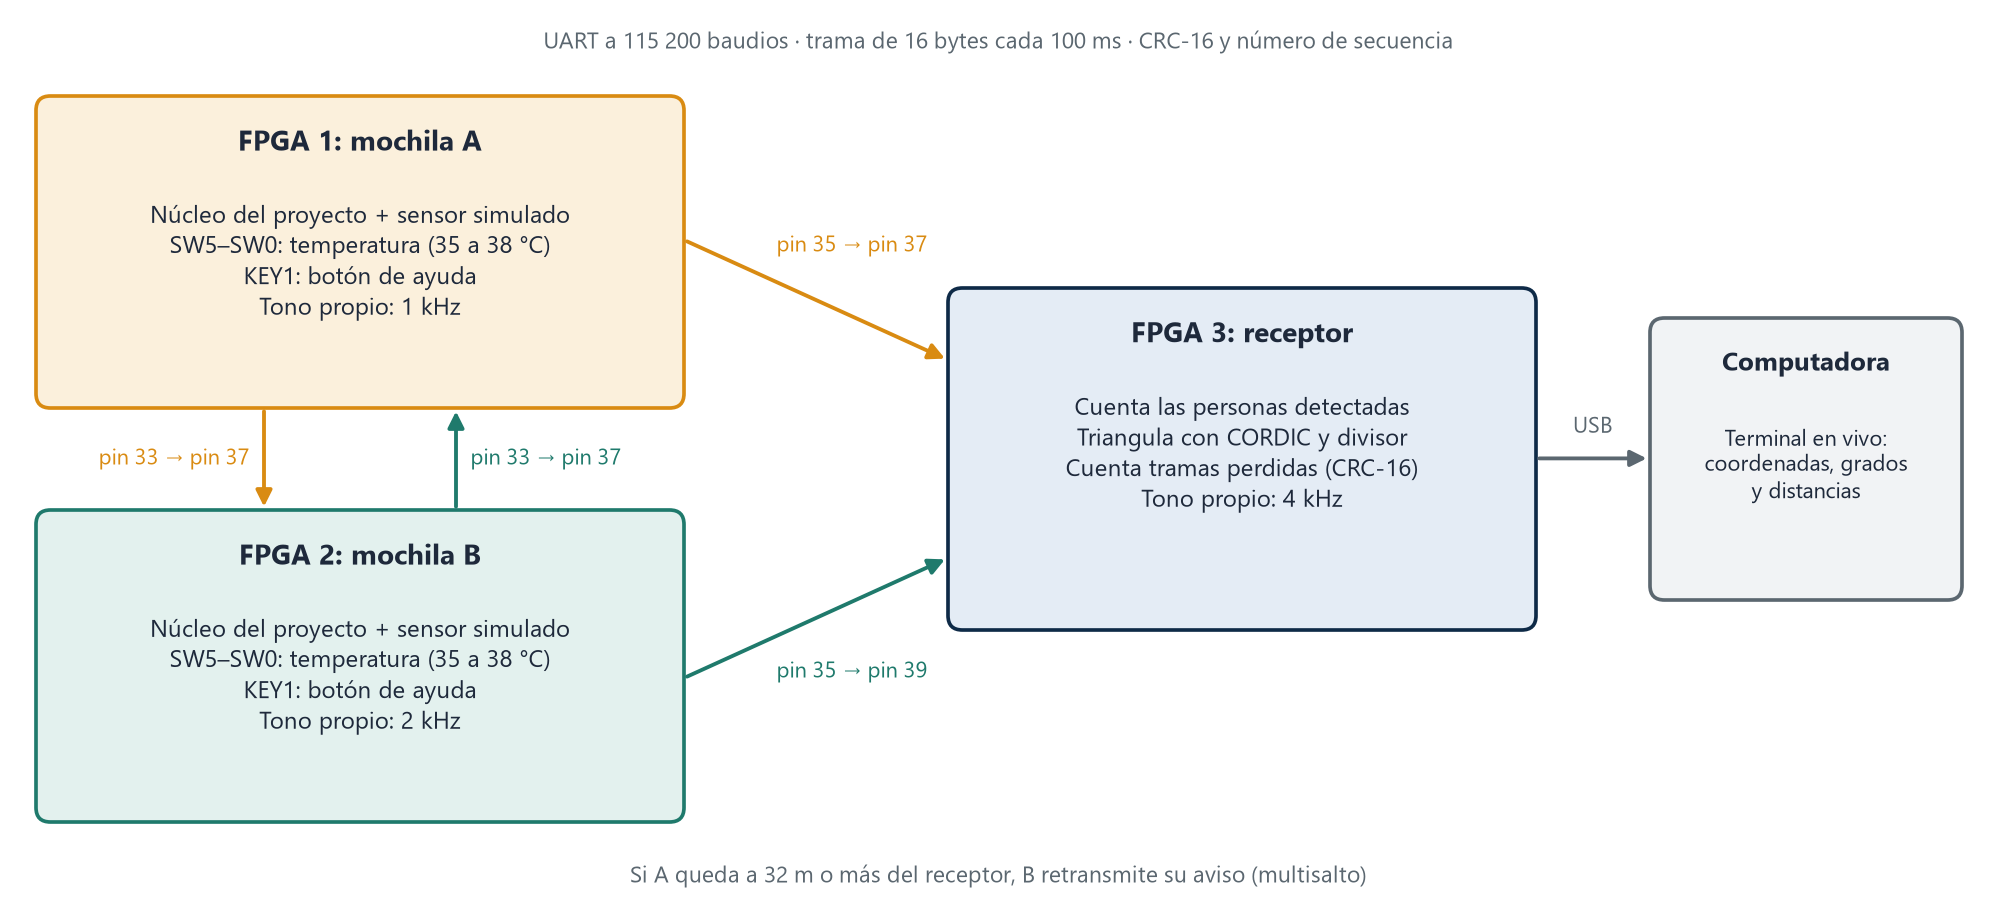
\includegraphics[width=\textwidth]{figs/red_tres_fpga.png}
\caption{Las tres tarjetas, sus enlaces por UART y la computadora del operador.}
\label{fig:tresfpga}
\end{figure}

\subsubsection{Qué hace cada nodo}

\begin{itemize}
  \item \textbf{Cada mochila} corre el núcleo de la sección~\ref{sec:nucleo}, sin cambiarle nada, sobre
        un sensor térmico simulado: los interruptores SW5--SW0 fijan, en grados y en binario, la
        temperatura que lee la matriz. Detecta a una persona de dos formas redundantes: por
        temperatura, entre 35 y 38~\textdegree C, y por el botón de ayuda que va sobre el insecto.
        Mide en qué dirección ve el calor, emite un tono propio, transmite su estado diez veces por
        segundo y retransmite una vez las tramas de la otra mochila.
  \item \textbf{El receptor} junta lo que llega, cuenta las personas detectadas, cruza los rumbos de
        las dos mochilas para estimar dónde está la persona y deja todo en registros que la
        computadora lee.
  \item \textbf{La computadora} muestra esos registros en una terminal y manda órdenes de prueba.
        No hace ninguna cuenta del sistema (tabla~\ref{tab:reparto}).
\end{itemize}

Los parámetros de la demostración son parámetros de los módulos, con nombre
(tabla~\ref{tab:parametrosred}).

\begin{table}[H]
\centering\footnotesize
\caption{Parámetros de la demostración y dónde están en el código.}
\label{tab:parametrosred}
\rowcolors{2}{SoftGray}{white}
\begin{tabularx}{\textwidth}{@{}>{\bfseries\raggedright\arraybackslash}p{3.6cm} >{\raggedright\arraybackslash}X >{\raggedright\arraybackslash}p{4.3cm}@{}}
\toprule
\rowcolor{TableHead} Parámetro & Valor & En el código \\
\midrule
Ventana de temperatura de una persona & 35 a 38~\textdegree C, las dos incluidas & \sig{T\_PERSONA\_MIN}, \sig{T\_PERSONA\_MAX} \\
Sensor térmico simulado & SW5--SW0: grados en binario, de 0 a 63 & \sig{sw[5:0]} de \sig{tri\_mochila} \\
Segunda detección & KEY1 sostenido 0.1~s; queda marcado hasta el reset & \sig{T\_PULSA\_MS} \\
Conteo de personas & 0, 1 o 2, igual en las tres tarjetas y en la terminal; baja si la temperatura sale de la ventana & \sig{cuenta\_pd}, \sig{REARMA} \\
Alcance del radio y de los tonos & Menos de 32~m: a 31~m se oye; a 32~m o más, no & \sig{ALCANCE\_M} \\
Escala de distancias & 10 bits, de 0 a 64~m: 6.25~cm por cuenta. Cinco metros son 80 cuentas, el 7.8~\% de la escala & \sig{tri\_distancia} \\
Tonos & A 1~kHz, B 2~kHz y receptor 4~kHz; umbral de potencia de 4\,000 & \sig{tri\_tonos}, \sig{UMBRAL} \\
Enlace & UART 8N1 a 115\,200 baudios; trama de 16 bytes cada 100~ms & \sig{BAUD\_RATE}, \sig{tri\_tx\_n}, \sig{tri\_rx\_n} \\
\bottomrule
\end{tabularx}
\end{table}

\subsubsection{Lo que se ve en cada tarjeta}

\begin{table}[H]
\centering\footnotesize
\caption{Displays y LED de la red. Un guion en HEX1 o HEX0 quiere decir que no se oye a ese nodo.}
\label{tab:displays}
\rowcolors{2}{SoftGray}{white}
\begin{tabularx}{0.92\textwidth}{@{}>{\bfseries\raggedright\arraybackslash}p{2.2cm} >{\raggedright\arraybackslash}X >{\raggedright\arraybackslash}X@{}}
\toprule
\rowcolor{TableHead} Indicador & En una mochila & En el receptor \\
\midrule
HEX5 & Quién es: \sig{A} o \sig{b} & \sig{r} \\
HEX4--HEX3 & \sig{Pd}, personas detectadas & \sig{Pd} \\
HEX2 & Cuántas: 0, 1 o 2 & Lo mismo \\
HEX1 & La letra de la otra mochila, si oye su tono & \sig{A}, si oye el tono de A \\
HEX0 & \sig{r}, si oye el tono del receptor & \sig{b}, si oye el tono de B \\
LEDR9--5 & Metros a la otra mochila, en binario & Metros a la mochila A \\
LEDR4--0 & Metros al receptor & Metros a la mochila B \\
\bottomrule
\end{tabularx}
\end{table}

Con cinco LED se cuentan hasta 31~m, que es justo el alcance. Los metros van sin redondear
(31.9~m marca 31), y un nodo que se oye marca al menos 1 aunque esté a menos de un metro: así,
los cinco LED apagados quieren decir siempre «no lo oigo».

\subsubsection{Mapa, escala y alcance}

Las posiciones van en 10 bits sobre un mapa de 0 a 64~m, de modo que una cuenta vale 6.25~cm.
El receptor está en $(0,0)$ y la persona en $(25.50,\,19.25)$~m, a 31.95~m: justo en el borde
del alcance. Por eso, de dos mochilas que están junto a la persona, una puede quedar dentro
del alcance y la otra fuera, y entonces la primera hace de puente (figura~\ref{fig:mapared}).

\begin{figure}[H]
\centering
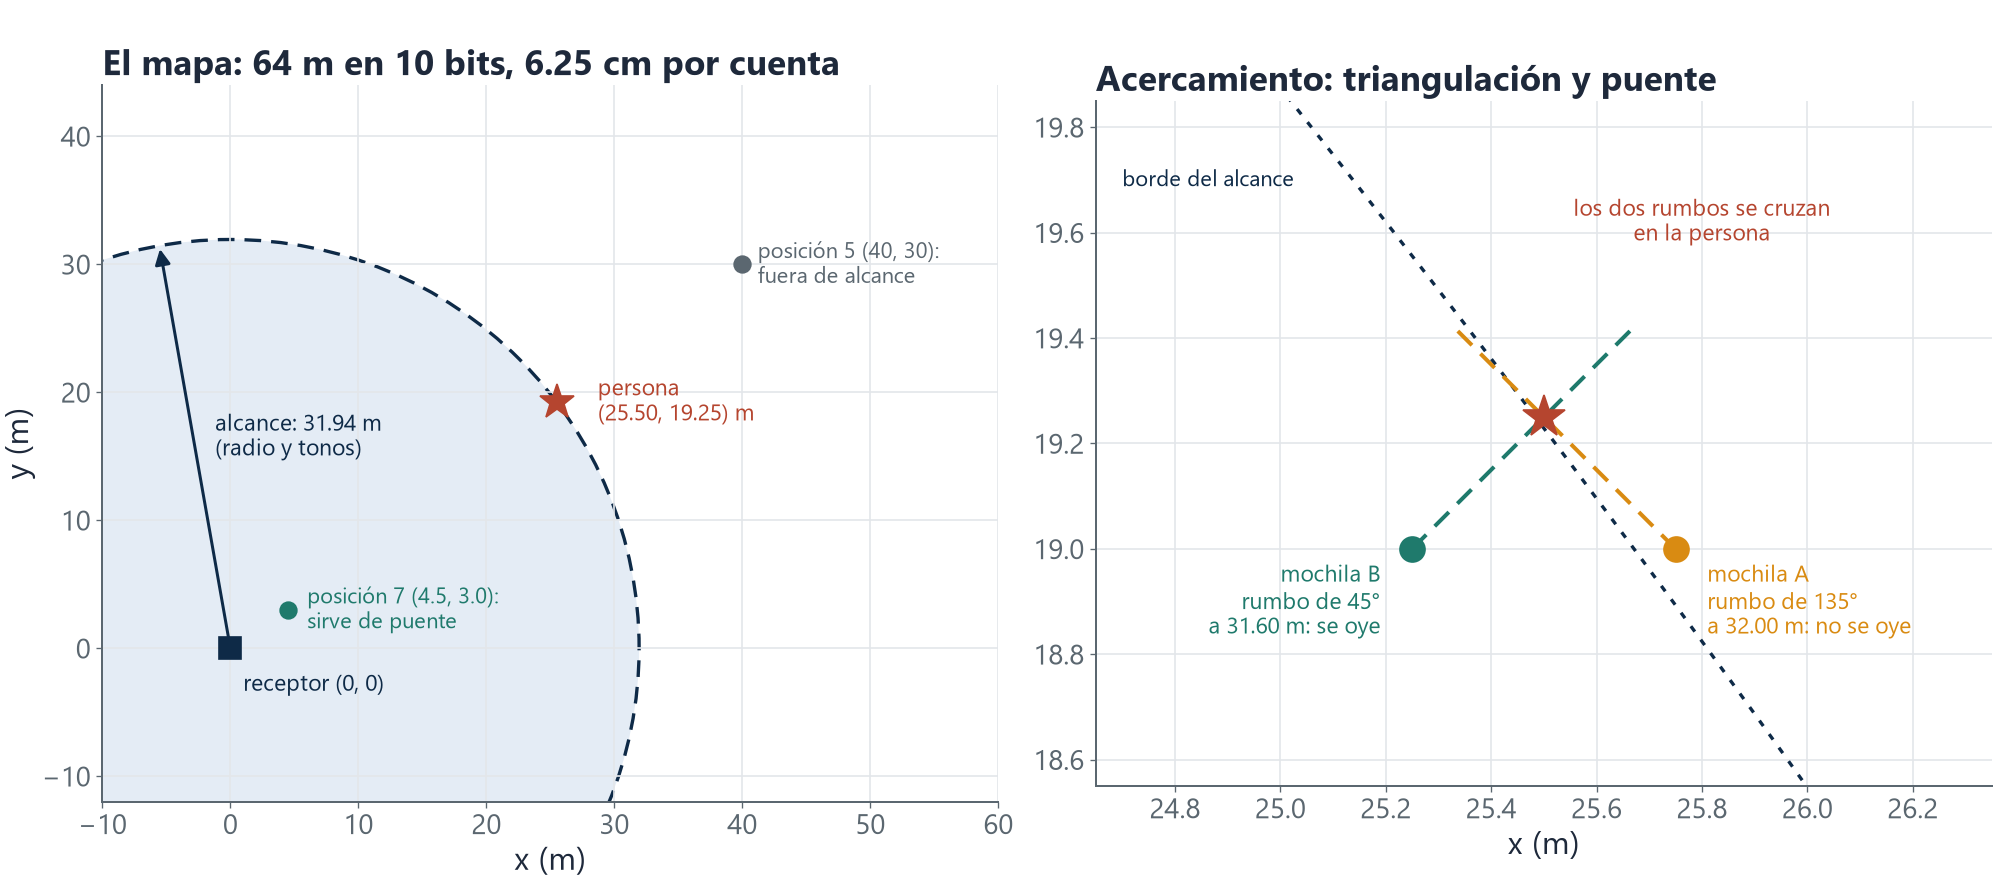
\includegraphics[width=\textwidth]{figs/red_mapa.png}
\caption{El mapa de 64~m con el alcance de 32~m, y el acercamiento donde se cruzan los dos rumbos.}
\label{fig:mapared}
\end{figure}

La distancia entre dos nodos se calcula exacta, con una raíz cuadrada entera
(sección~\ref{sec:raiz}), y la regla del alcance usa la misma suma de cuadrados:
\begin{equation}
d=\left\lfloor\sqrt{\Delta x^2+\Delta y^2}\,\right\rfloor\ \text{cuentas},\qquad
\text{se oye si}\quad \Delta x^2+\Delta y^2<(16\times32)^2 .
\label{eq:alcance}
\end{equation}
Como las dos salen del mismo número, no pueden contradecirse: un nodo se oye exactamente
cuando su distancia marca menos de 32.00~m.

\subsubsection{Protocolo de enlace}

El enlace es UART 8N1 a 115\,200 baudios, el de la práctica~4, con una trama propia de 16 bytes
que cada mochila transmite cada 100~ms (figura~\ref{fig:trama}).

\begin{figure}[H]
\centering
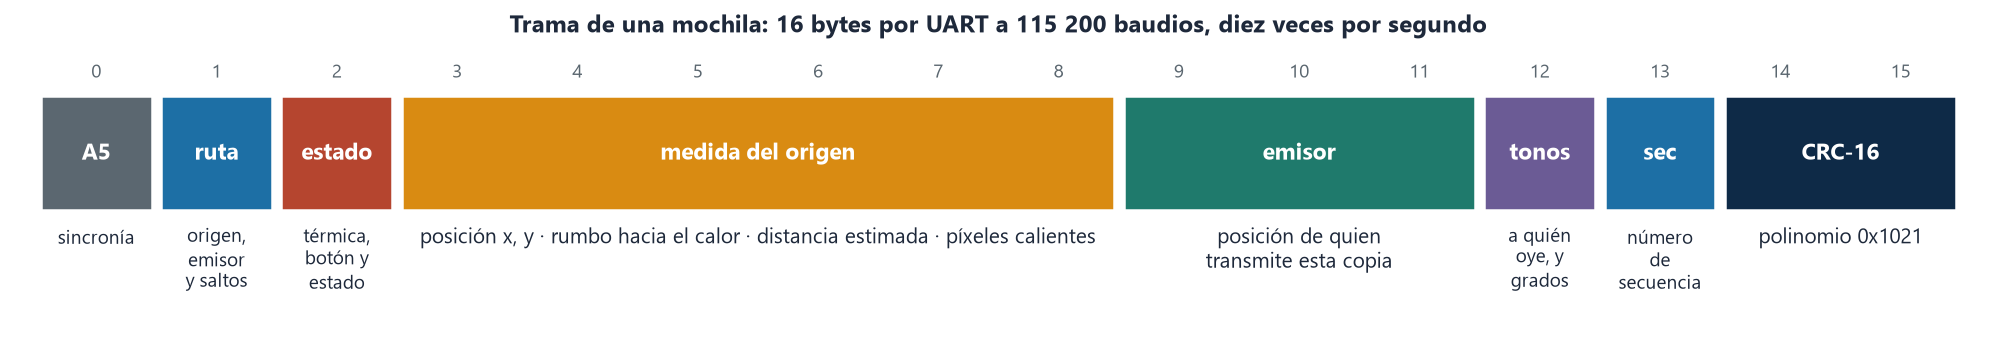
\includegraphics[width=\textwidth]{figs/red_trama.png}
\caption{Los 16 bytes de la trama de una mochila.}
\label{fig:trama}
\end{figure}

El byte de ruta distingue al \emph{origen}, la mochila que midió, del \emph{emisor}, la que
transmite esta copia. Quien recibe aplica cinco reglas:
\begin{itemize}
  \item Descarta la trama si el CRC-16 no coincide o si se interrumpe más de 2~ms. El CRC usa el
        polinomio \sig{0x1021} con valor inicial \sig{0xFFFF} sobre los bytes 1 a 13; un código
        cíclico de 16 bits detecta toda ráfaga de errores de 16 bits o menos~\cite{peterson1961}.
  \item Solo la acepta si el emisor está a menos de 32~m: así se simula el alcance del radio.
  \item Una mochila reenvía una sola vez las tramas de la otra, con el contador de saltos
        incrementado. Es lo que permite el puente.
  \item Con el número de secuencia, el receptor cuenta las tramas perdidas y reconoce la que le
        llega repetida por dos caminos.
  \item Si en un segundo no llega nada de una mochila, la da por perdida.
\end{itemize}

\subsubsection{Reconocer a los vecinos por tonos}

La radio dice qué mide cada mochila, pero no quién le queda cerca. Para eso cada nodo emite todo
el tiempo un tono distinto (A 1~kHz, B 2~kHz y el receptor 4~kHz) y escucha los otros dos: con
saber a quién oye, sabe quién está a su alcance, sin conocer su posición. Cada nodo muestrea su
micrófono a 16~kHz y, cada 64 muestras (4~ms), tres filtros de Goertzel~\cite{goertzel1958}
miden la potencia en las tres frecuencias (sección~\ref{sec:goertzel}). Un tono se da por oído
si su potencia pasa del umbral en dos bloques seguidos, y por perdido si queda debajo en dos.

En la demostración no hay bocinas ni micrófonos. El canal acústico va simulado dentro de la
FPGA: la señal del micrófono es la suma de las ondas cuadradas de los nodos que están a menos
de 32~m, más ruido, y los filtros trabajan sobre esa señal como lo harían sobre la real. Para
probarlo con hardware bastan dos cambios, y ninguno toca los filtros: el tono propio ya sale
por el pin~1 del conector JP1, listo para un zumbador, y la suma simulada se sustituye por las
muestras de un micrófono con su convertidor.

\subsubsection{Rumbo y triangulación}

Cada mochila mide el rumbo hacia el calor: el centroide de las columnas calientes de la matriz,
que da el ángulo respecto al frente del insecto, más el rumbo del insecto. El receptor cruza las
dos rectas que salen de A y de B con esos rumbos:
\begin{equation}
P=A+t\,\hat u_A,\qquad t=\frac{(B-A)\times\hat u_B}{\hat u_A\times\hat u_B},
\qquad \hat u=(\cos\theta,\ \sin\theta).
\label{eq:triangula}
\end{equation}
Los cosenos y senos salen de un CORDIC en rotación y el cociente de un divisor con restauración
(sección~\ref{sec:cordic}); no hay tablas de seno ni funciones de biblioteca. El módulo distingue
tres casos en los que el cruce no sirve y lo indica: rumbos casi paralelos (menos de
10\textdegree{} entre sí), rectas que se cruzan detrás de una mochila y cruce a más de 3~m. En
esos casos, o si solo una mochila detecta, el receptor usa la aproximación de cada mochila por
separado: su posición más la distancia que estima por el tamaño de la mancha.

\textbf{El sensor simulado no altera el núcleo.} El módulo \sig{tri\_escena} conoce la posición
de la persona; con la posición y el rumbo del insecto calcula, con un CORDIC en vectorización,
en qué columna de la matriz caería la mancha, y entrega los 64 píxeles con la temperatura de
los interruptores sobre un fondo de 22~\textdegree C. El núcleo recibe esos píxeles como los
recibiría del sensor.

\subsubsection{Reparto entre la FPGA y la computadora}

\begin{table}[H]
\centering\footnotesize
\caption{Dónde corre cada función del sistema.}
\label{tab:reparto}
\rowcolors{2}{SoftGray}{white}
\begin{tabularx}{0.9\textwidth}{@{}>{\raggedright\arraybackslash}X >{\raggedright\arraybackslash}p{4.2cm}@{}}
\toprule
\rowcolor{TableHead} \textbf{Función} & \textbf{Dónde corre} \\
\midrule
Detección térmica, filtrado, decisión y estímulo & FPGA (mochila) \\
Rumbo hacia el calor & FPGA (mochila) \\
Tramas, CRC-16, número de secuencia, alcance y puente & FPGA (las tres) \\
Generación y detección de tonos & FPGA (las tres) \\
Distancias exactas entre nodos & FPGA (las tres) \\
Conteo de personas y triangulación & FPGA (receptor) \\
Displays y LED & FPGA (las tres) \\
Mostrar los datos y mandar órdenes de prueba & Computadora \\
\bottomrule
\end{tabularx}
\end{table}

La computadora lee por el cable USB-Blaster los registros del receptor, con una sonda de
Quartus (\emph{In-System Sources and Probes}~\cite{intelissp}), los convierte a metros y grados
y los escribe en pantalla; no hace falta ningún adaptador serie. Por la misma sonda puede
fijar la posición y la temperatura de cada mochila, que es como se prueban el alcance y el
puente sin mover cables. Si la computadora se desconecta, las tres tarjetas siguen funcionando
igual: los displays y los LED no dependen de ella.
